\documentclass[12px]{article}

\title{Lezione 6 Algebra I}
\date{2024-10-21}
\author{Federico De Sisti}

\input{../../../setup.tex}

\begin{document}
	\maketitle
	\newpage
	\section{Teoremi sulla cardinalità dei gruppi}
	\begin{teo}
		
	$(G,\cdot)$ gruppo. Se $|G| = 6$ allora\\
	 $G\cong C_6$ (abeliano) oppure $G\cong D_3$ (non abeliano)
	\end{teo}
	\begin{dimo}
		Se $G$ contiene un elemento di ordine 6 allora $G\cong C_6$\\
		Se invece $G$ non contiene elementi di  ordine 6, per l'esercizio (2) esistono elementi $r,s\in G$ t.c. $ord(r) = 3$ e $ord(s) = 2$\\
		Definisco:\\
		\[
			G:=<r>=\{e,r,r^2\} \ \ \ \ k:=<s>=\{e,s\}
		.\] 
		\[
			H\cap K = \{e\}
		.\] 
		\[
			|HK| = \frac{|H||K|}{|H\cap K |} = 6 = |KH|
		.\] 
		$ \Rightarrow HK = G = KH$ \\
		\textbf{Esplicitamente:}\\
		$HK = \{e,r,r^2,s,rs,r^2s\}$\\
		$KH = \{e,r,r^2,s,sr,sr^2\}$\\
		 \textbf{Dobbiamo considerare 2 casi:}\\
		 I caso:  $rs = sr$\\
		 studiamo  $ord(rs)$\\
		  $(rs)^2 = r^2s^2 = r^2\neq e \Rightarrow ord(rs)\neq 2$ \\
		  $(rs)^3 = r^3s^3 = s^3 = s\neq e$\\
		  \textbf{Per Lagrange}\\
		   necessariamente $ord(rs) = 6$\\
		    $ \Rightarrow G$ è cicliclo $ \Rightarrow  $ Assurdo\\
		    II caso:
		    \begin{cases}
		    	rs = sr^2\\
			r^2s = sr
		    \end{cases}\\
		    Costruiamo l'isomorfismo\\
		    \begin{gather*}
		    	G \rightarrow D_3:=<\rho,\sigma>\\
			e \rightarrow Id\\
			r \rightarrow \rho\\
			r^2 \rightarrow \rho^2\\
			s \rightarrow \sigma\\
			sr \rightarrow \sigma\rho
		    \end{gather*}
	\end{dimo}
	\begin{defi}
		Dato un gruppo $(G,\cdot)$ il reticolo dei sottogruppi $T_G$ è un grafo definito come\\
		\begin{itemize}
			\item esiste un vertice in $T_G$ per ogni sottogruppo $H\leq G$ \\
			\item esiste un lato $H_1$ \---- $H_2$ se e solo se $H_1\subseteq H_2$ \\e $\cancel\exists K\leq G$ t.c. $H_1\subset K\subset H_2$
		\end{itemize}
	\end{defi}
	\textbf{Esempio:}\\
	$T_{D_4}$\\
	Ricordiamo che $D_4 = <\sigma,\rho>  \ \ |D_4|=8$\\
	studiamo i sottogruppi di $D_4$\\
	\textbf{ordine 1:} L'unico sottogruppo è $H=\{e\}$\\
	 \textbf{ordine 2:} Sono tutti e soli quelli generati da un elemento di ordine $2$ in $D_4$
	 \begin{center}
	 \begin{tikzpicture}
    % Nodes
    \node (A) at (0,0) {$\langle \sigma \rangle$};
    \node (B) at (2,0) {$\langle \sigma \rho \rangle$};
    \node (C) at (4,0) {$\langle \rho^2 \rangle$};
    \node (D) at (6,0) {$\langle \sigma \rho^2 \rangle$};
    \node (E) at (8,0) {$\langle \sigma \rho^3 \rangle$};
    \node (F) at (4,-1) {$\{e\}$}$

    % Arrows
    \draw[-] (A) -- (F);
    \draw[-] (B) -- (F);
    \draw[-] (C) -- (F);
    \draw[-] (D) -- (F);
    \draw[-] (E) -- (F);
\end{tikzpicture}
	 \end{center}
	 \textbf{ordine 4:} per la classificazione sono ciclici $(C_4)$ oppure di Klein $(K_4)$ altre al ciclico $<p>$ esistono altri sottogruppi\\
	 \[
		 \langle \rho^2,\sigma\rangle = \{e, \sigma,\rho^2,\sigma\rho^2\}
	 .\] 
	 \[
		 \rangle\rho^2, \sigma\rho\rangle = \{e,\sigma\rho, \rho^2,\sigma\rho^3\}
	 .\]
	 Ordine 8: $D_4$\\
	 \begin{center}
	 \begin{tikzpicture}
    % Nodes
    \node (A) at (4,0) {$\langle \sigma, \rho \rangle$};
    \node (B) at (2,-2) {$\langle \sigma\rho^2 \rangle$};
    \node (C) at (4,-2) {$\langle \rho \rangle$};
    \node (D) at (6,-2) {$\langle \sigma, \rho^2 \rangle$};
    \node (E) at (0,-4) {$\langle \sigma\rho^3 \rangle$};
    \node (F) at (2,-4) {$\langle \sigma\rho \rangle$};
    \node (G) at (4,-4) {$\langle \rho^2 \rangle$};
    \node (H) at (6,-4) {$\langle \sigma\rho^2 \rangle$};
    \node (I) at (8,-4) {$\langle \sigma \rangle$};
    \node (J) at (4,-6) {$\lbrace e \rbrace$};


    % Arrows
    \draw[-] (A) -- (B);
    \draw[-] (A) -- (C);
    \draw[-] (A) -- (D);
    \draw[-] (B) -- (E);
    \draw[-] (B) -- (F);
    \draw[-] (B) -- (G);
    \draw[-] (C) -- (G);
    \draw[-] (D) -- (G);
    \draw[-] (D) -- (H);
    \draw[-] (D) -- (I);
    \draw[-] (E) -- (J);
    \draw[-] (F) -- (J);
    \draw[-] (G) -- (J);
    \draw[-] (H) -- (J);
    \draw[-] (I) -- (J);

\end{tikzpicture}
	 \end{center}
	 \textbf{Esempio:}\\
	 $G=D_4\\
	 N=<\rho^2>\trianglelefteq G$\\
	 Vogliamo $T_{G/N}$\\
	 studiamo $G/N = D_4/<rho^2>$\\
	 $\displaystyle|G/N| = [G:N] = \frac {|G|}{|N|} = \frac 82 = 4$\\
	 chi sono i laterali?\\
	 $IdN = N <\rho^2> = \{Id,\rho^2\}$\\
	 $\rho N = \{\rho, \rho ^3\}$\\
	 $\sigma N = \{\sigma, \sigma \rho^2\}$\\
	 $\sigma\rho N = \{\sigma\rho, \sigma\rho^3\}$\\
	  \textbf{Ricordo:}\\
	  Abbiamo una corrispondenza biunivoca tr ai sottogruppi di $G/N$ e i sottogruppi di $G$ contenenti $N$.\\
	  \begin{center}
	  	
	  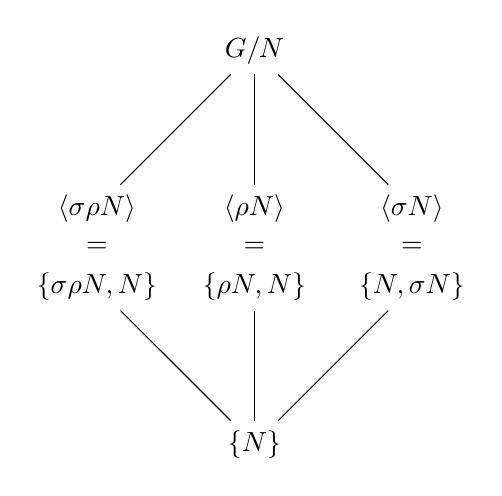
\begin{tikzpicture}
    \node (A) at (4,0) {$G/N$};
    \node (B) at (2,-2) {$\langle\sigma\rho N\rangle$};
    \node (C) at (4,-2) {$\langle\rho N\rangle$};
    \node (D) at (6,-2) {$\langle\sigma N\rangle$};
    \node (E) at (2,-3) {$\{\sigma\rho N, N\}$};
    \node (F) at (4,-3) {$\{\rho N, N\}$};
    \node (G) at (6,-3) {$\{N, \sigma N\}$};
    \node (H) at (4,-5) {$\{N\}$};
    
    \draw[-] (A) -- (B);
    \draw[-] (A) -- (C);
    \draw[-] (A) -- (D);
    \path (B)--(E) node[midway]{\storto =};
    \path (C)--(F) node[midway]{\storto =};
    \path (D)--(G) node[midway]{\storto =};
    \draw[-] (E) -- (H);
    \draw[-] (F) -- (H);
    \draw[-] (G) -- (H);
	  \end{tikzpicture}
	  \end{center}
	  \textbf{Obiettivo: studiare $S_n$}\\
	  \textbf{Ricordo:}\\
	  $X:=\{1,\ldots,n\}$\\
	  $S_n:=S_X= \{$ applicazioni biunivoche $X \rightarrow X\}$\\
	  $S_n$ gruppo di permutazioni\\
	   \textbf{Osservazione:}\\
	   $|S_n| = n!$\\
	   \textbf{Osservazione:}\\
	   se $n=3 \rightarrow |S_3| = 6$\\
	   $ \Rightarrow S_3 \cong D_3$ \\
	   \textbf{Osservazione}\\
	   $S_n\cong D_n \ \ \forall n\geq 4$\\
	   Infatti  $n! > 2n \ \ \forall n\geq 4$ 
	   \section{Notazioni in $S_n$}\\
	   \begin{aligend*}
	   	\sigma = (1 2 3)(4 7)\\
	   	\tau = (23456)\\
		\sigma\tau=\sigma\circ\tau = (123)(46)(23456)(12)(36)(45)\\
		\tau\circ\sigma = (23456)(123)(46) = (13)(24)(56)

	   \end{aligend*}
	   \begin{lemm}
		   Data $\sigma\in S_n$ allora  $\sigma$ partizione $X = \{1,\ldots, n\}$ in sottoinsiemi permutati ciclicamente e disgiunti tra loro
	   \end{lemm}
	   \begin{dimo}
	   	Definiamo la relazione d'equivalenza $i\sim j \Leftrightarrow \exists k\in \mathbb Z \ t.c. \ \sigma^k(i) = j$\\
		È una relazione d'equivalenza!\\
		\textbf{studiamo le classi di equivalenza}\\
		fissato $i\in X$\\
		la sua clase
		 \[
			 X_i = \{\sigma^k(i)|k\in \mathbb Z\}\subseteq X
		.\] 
	quindi $\exists \ \ k_1,k_2\in \mathbb Z$ distinti t.c. $\sigma^{k_1}(i) = \sigma^{k_2}(i)$\\
	\begin{aligned*}
		\Rightarrow i = \sigma^{k_2-k_1}(i)\\
		\Rightarrow m:=min\{k\in\mathbb Z_{>0}|\sigma^k(i) = i\}\\
		\Rightarrow X_i = \{i,\sigma(i),\sigma^2(i),\ldots,\sigma^{n-1}(i)\}
	\end{aligned*}
	   \end{dimo}
	\begin{prop}
		Data $\sigma\in S_n$, allora  $\sigma$ può essere rappresentata come composizione di cicli disgiunti
	\end{prop}
	\textbf{Obiettivo:}
		Definire un omomorfismo
		\[
			sgn: S_n \rightarrow (\{\pm 1\}, \cdot)
		.\] 
		Questo ci permetterà di definire  il sottogruppo  alterno $A_n\trianglelefteq S_n$\\
		$A_n:=ker(sgn)$
		\newpage
	\begin{nota}
		Dato un polinomio\\
		$f\in \mathbb Q[x_1,\ldots, x_n]$\\
		e data $\sigma\in S_n$\\
		Definiamo
		 \[
			 f^\sigma (x_1,\ldots,x_n) := f(x_{\sigma(1),\ldots,x_{\sigma(n)\}
		.\]
		Ci sta un polinomio speciale:\\
		\begin{itemize}
			\item $\Delta (x_1,\ldots, x_n) = \prod_{1\leq i< j\leq n}(x_i - x_j)$
				\item $\Delta^\sigma (x_1,\ldots, x_n) = \prod_{1\leq i< j\leq n} (x_{\sigma (i)} - x_{\sigma (j)})$
		\end{itemize}
	\end{nota}
	\begin{defi}
		$\sigma\in S_n$\\
		$sgn(\sigma) := \frac {\Delta^\sigma}\Delta\in\{\pm 1\}$\\
	\end{defi}
		 \textbf{Osservazione}\\
		 $sgn: S_n \rightarrow \{\pm 1\}$ \\
		 è un omomorfismo\\
		 \begin{dimo}
		 	In generale\\
			$(f^\sigma)^\tau = f^{\sigma\tau}$\\
			 $(fg)^\sigma = f^\sigma g^\sigma$\\
			 $\displaystyle sgn(\sigma\tau)=\frac {\Delta^{\delta\tau}}\Delta = \frac {(\Delta^\sigma)^\tau)} \Delta = \frac {\Delta^\sigma}{\Delta} \frac {(\Delta^\sigma)^\tau}{\Delta^\sigma} = sgn(\sigma)\frac{\Delta^\tau}\Delta = sgn(\delta)sgn(\tau)$
		 \end{dimo}




	 \end{document}
